% --------------------------------------------------------------
%     DENNE MALEN ER LAGET AV MARTIN SORIA RØVANG
%     TIL BRUK FOR OPPGAVELØSNINGER OG RAPPPRTER
%     GITHUB: github.com/martinrovang
% --------------------------------------------------------------


\documentclass[10pt]{article}
\usepackage{amsmath,amsthm,amssymb}
\usepackage{float}
\usepackage[norsk]{babel}
\usepackage[table]{xcolor}
\usepackage{color}
\usepackage{graphicx}
\usepackage{listings}
\usepackage{natbib}
\usepackage[utf8]{inputenc}
\usepackage{imakeidx}
\usepackage[a4paper]{geometry}
\usepackage[myheadings]{fullpage}
\usepackage{fancyhdr}
\usepackage{lastpage}
\usepackage{graphicx, wrapfig, subcaption, setspace, booktabs}
\usepackage[T1]{fontenc}
\usepackage[font=small, labelfont=bf]{caption}
\usepackage{fourier}
\usepackage[protrusion=true, expansion=true]{microtype}
\usepackage{url, lipsum}
\usepackage{tgbonum}
\usepackage{hyperref}
\usepackage{xcolor}
\usepackage[most]{tcolorbox}
\usepackage{mathtools}
\usepackage[page]{totalcount}
\usepackage{lastpage}


\newcommand{\HRule}[1]{\rule{\linewidth}{#1}}
\onehalfspacing
\setcounter{tocdepth}{5}
\setcounter{secnumdepth}{5}
\newcommand{\vect}[1]{\boldsymbol{#1}}

\definecolor{codegreen}{rgb}{0,0.6,0}
\definecolor{codegray}{rgb}{0.5,0.5,0.5}
\definecolor{codepurple}{rgb}{0.58,0,0.82}
%\definecolor{backcolour}{rgb}{0.95,0.95,0.92}
\definecolor{skyblue}{rgb}{0.950, 1, 1}
\definecolor{pink}{rgb}{1, 0.1, 0.5}

\lstdefinestyle{mystyle}{
    backgroundcolor=\color{skyblue},   
    commentstyle=\color{codegreen},
    keywordstyle=\color{magenta},
    numberstyle=\tiny\color{codegray},
    stringstyle=\color{codepurple},
    basicstyle=\footnotesize,
    breakatwhitespace=false,         
    breaklines=true,                 
    captionpos=b,                    
    keepspaces=true,                 
    numbers=left,                    
    numbersep=5pt,                  
    showspaces=false,                
    showstringspaces=false,
    showtabs=false,                  
    tabsize=2,
    frame=single,
    %keywordstyle=\color{blue},
    language=Python
}
 
\lstset{style=mystyle}
\lstset{
    basicstyle=\footnotesize\ttfamily,
  identifierstyle=\bfseries\color{pink!40!pink},
  commentstyle=\itshape\color{black!40!black},
  keywordstyle=\color{blue},
  stringstyle=\color{orange},
}

\newcommand{\N}{\mathbb{N}}
\newcommand{\Z}{\mathbb{Z}}
 
\newenvironment{theorem}[2][Theorem]{\begin{trivlist}
\item[\hskip \labelsep {\bfseries #1}\hskip \labelsep {\bfseries #2.}]}{\end{trivlist}}
\newenvironment{lemma}[2][Lemma]{\begin{trivlist}
\item[\hskip \labelsep {\bfseries #1}\hskip \labelsep {\bfseries #2.}]}{\end{trivlist}}
\newenvironment{exercise}[2][Exercise]{\begin{trivlist}
\item[\hskip \labelsep {\bfseries #1}\hskip \labelsep {\bfseries #2.}]}{\end{trivlist}}
\newenvironment{problem}[2][Problem]{\begin{trivlist}
\item[\hskip \labelsep {\bfseries #1}\hskip \labelsep {\bfseries #2.}]}{\end{trivlist}}
\newenvironment{question}[2][Question]{\begin{trivlist}
\item[\hskip \labelsep {\bfseries #1}\hskip \labelsep {\bfseries #2.}]}{\end{trivlist}}
\newenvironment{corollary}[2][Corollary]{\begin{trivlist}
\item[\hskip \labelsep {\bfseries #1}\hskip \labelsep {\bfseries #2.}]}{\end{trivlist}}

\newenvironment{solution}{\begin{proof}[Solution]}{\end{proof}}
    
\makeindex[columns=3, title=Alphabetical Index, intoc]


% --------------------------------------------------------------
%                         Headers and footers
% --------------------------------------------------------------
\fancyhf{}
\pagestyle{fancy}
\rhead{Martin Soria Røvang}
\lhead{INF-1400-Objektorientert programmering}
\rfoot{Side \thepage \, av \pageref{LastPage}}
\renewcommand{\headrulewidth}{0.3pt}



\begin{document}
% --------------------------------------------------------------
%                         FRONTPAGE
% --------------------------------------------------------------
{\fontfamily{cmr}\selectfont
\title{ \normalsize \textsc{}
		\\ [3.0cm] % How much upper margin
		%\HRule{0.5pt} \\
        \LARGE \textbf{\uppercase{Rapport Oppgave 2}
        \HRule{0.5pt} \\ [0.5cm]
        INF-1400-Objektorientert programmering
        %\HRule{2pt} \\ [0.5cm]
        \\
		\normalsize \today \vspace*{5\baselineskip}}
		}

        \date{}
\author{
		Martin Soria Røvang \\ 
        Universitetet i Tromsø \\}

% \begin{titlepage}
\clearpage\maketitle
\vspace{0.2\textheight}
{\centering
Inneholder \pageref{LastPage} \, sider, inkludert forside.\par
}
\thispagestyle{empty}
% \end{titlepage}

\newpage
\tableofcontents
% --------------------------------------------------------------
%                         Start here
% --------------------------------------------------------------


\newpage

\section{Introduksjon}

\subsection{Krav}


\section{Teknisk bakgrunn}
ARV \\
super

\section{Design}
\subsection{Klassestruktur}
I dette prosjektet har vi klassestrukturen som vist i figur(\ref{klassestrukturen}) under,
\begin{figure}[hbt!]
{\centering
    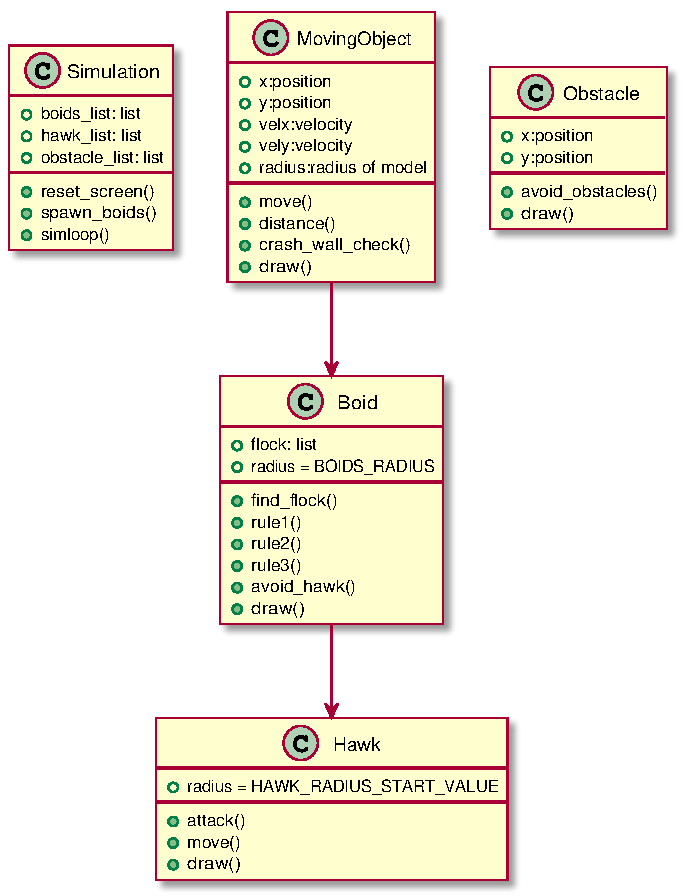
\includegraphics[width=0.50\textwidth]{classes.pdf}
    \caption{Klassestrukturen i programmet.}
    \label{klassestrukturen}
\par}
\end{figure}

Her arver \emph{Boid} klassen fra \emph{MovingObject} og \emph{Hawk}(Hoik) fra Boid. Hvis man arver fra en generell struktur kan man spare kodeplass og generelt får mer strukturert kode. Hvis man arver fra en klasse får man alle metodene og attributtene fra klassen man arver fra. I noen av klassene ble noen av metodene og attributter erstattet. Dette ble gjort ved å lage en metode som heter det samme i barneklassen(den klassen som arver). Dette gjelder også \emph{\_\_init\_\_()} metoden, derfor vil det oppstå problemer hvis man vil legge inn nye initialattributter, da dette vil erstatte arv-attributtene. et eksempel vil være å gjøre slik som vist i figur(\ref{nye_att})

\begin{figure}[hbt!]
    \begin{lstlisting}
        class eksempel:
            def __init__(self):
                super().__init__()
                self.a = 10
    \end{lstlisting}
\caption{Lage nye initialattributter og hente de andre fra foreldreklassen}
\label{nye_att}
\end{figure}

\subsection{Simulation}

Simulation er klassen som styrer hva som skal kjøres i programmet. Den har følgene metoder,\\

\begin{itemize}
    \item \emph{reset\_screen}: Fyller skjermen med svart for å overskrive tidligere posisjoner.
    \item \emph{spawn\_boids}: Lager boids hvis man trykker på venstre museknapp.
    \item \emph{simloop}: Dette er den metoden som kjører kontinuerlig i en while-loop så lenge simulasjonsprogrammet er på.
\end{itemize}

\subsection{MovingObject}

MovingObject er en generell funksjon som lager instanser som skal kunne bevege seg, finne distanser til andre bevegelige objekter, unngå å kræsje i vegger og tegne dem.
Dette er en klasse man vil arve fra når man skal ha mer spesifikke klasser som bruker alle/mange av metodene og attributtene til MovingObject.
MovingObject består av funksjonene,

\begin{itemize}
    \item \emph{move}: Beveger objektet etter hvor stor hastigheten er.
    \item \emph{distance}: Returnerer distansen til et annet objekt.
    \item \emph{crash\_wall\_check}: Sjekker om objektet er på vei utafor skjermen. Hvis objektet er på vei ut vil hastigheten bli reflektert og demped. Dette skjer ved å gange hastigheten $\vect{v}$ med en refleksjonskonstant gitt i konfigurasjonefilen.
    \item \emph{draw}: Tegner objektet ut på skjermen.
\end{itemize}

\emph{Move} metoden summer på den tidligere posisjonen og på en enhetsvektor som er skalert av verdi gitt fra konfigurasjonsfilen.

\begin{equation}
    \vect{V} = \frac{\vect{v}}{||\vect{v}||}\alpha
\end{equation}
,der $\alpha$ er en skalar for hva farten skal være slik at,
\begin{equation}
     ||\vect{V}|| = \alpha, \, \forall\,t
\end{equation}

Metoden \emph{distance} finner distansen til et annet objekt ved ta lengden gitt fra pytagoras,

\begin{equation*}
    Distance = \sqrt{(x_{2} - x_{1})^2 + (y_{2} - y_{1})^2}
\end{equation*}

der subindeks $\{1\}$ angir posisjonen til objektet man vil finne lengden fra og $\{2\}$ er posisjonen til objektet man vil finne lengden til.

\subsection{Boid}

Denne klassen inneholder metodene som får objektene til å oppføre seg som en naturlig flokk. Dette blir gjort ved å lage 3 forskjellige regler som kjører kontinuerlig i while-loopen i simulasjons-løkka. Denne klassen arver også fra \emph{MovingObject} derfor vil denne også inneholde alt den også har. Vi har metodene,

\begin{itemize}
    \item \emph{find\_flock}: Putter alle boidsene som tilhører en boid sin flokk i en liste som attributt til en boid. Alle boids vil derfor få en liste med boids(denne tar ikke med boidsen selv).
    \item \emph{rule1}: Finner gjennomsnitts-posisjonen og lager en vektor dit, denne blir summet på hastighetsvektoren til boidsen.
    \item \emph{rule2}: Boidsene unngår å kræsje i hverandre ved å summe på en vektor som er i motsatt retning av boidsen som den er på vei å kræsje med.
    \item \emph{rule3}: Boidsene prøver å matche hastigheten til boidsene som er i sin umiddelbare nærhet.\footnote{Disse reglene ble laget ved bruk av informasjonen på \url{http://www.kfish.org/boids/pseudocode.html}}
    \item \emph{avoid\_hawk}: Summer på vektor som er i motsatt retning av haukene/hoikene slik at de prøver å unngå dem.
    \item \emph{draw}: Tegner dem ut på skjermen.
\end{itemize}

I figur(\ref{rules}) ser man hvordan de tre vektorene kan se ut for en boid.
\begin{figure}[hbt!]
{\centering
    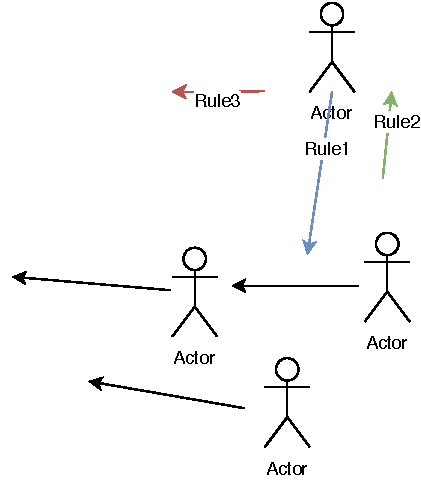
\includegraphics[width=0.30\textwidth]{rules.pdf}
    \caption{De forskjellige vektorene fra regel 1,2 og 3}
    \label{rules}
\par}
\end{figure}

Når disse blir summet opp vil man få en totalvektor som vist i figur(\ref{sumvektor}) under,

\begin{figure}[hbt!]
{\centering
    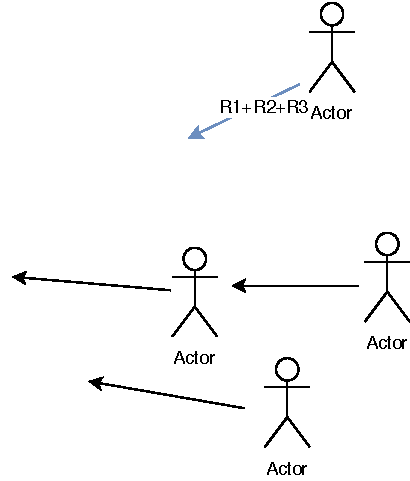
\includegraphics[width=0.30\textwidth]{rulelast.pdf}
    \caption{Summen av vektorene}
    \label{sumvektor}
\par}
\end{figure}

Dette gir en fin og glatt bevegelse til flokkene som ser noe naturlig ut.


\subsection{Hawk}

Denne klassen arver fra boids så disse vil oppføre seg likt som dem. Metodene er,

\begin{itemize}
    \item \emph{attack}: Summer opp hastighets-vektoren til hauken som peker i retningen av den nærmeste boiden.
    \item \emph{move}: Lagt til en egen move funksjon fordi hauken har en egen global variabel i konfigurasjonefilen som angir farten uavhengig av boid farten.
    \item \emph{draw}: Tegner hauken ut på skjermen.
\end{itemize}


Denne klassen var ganske grei å implementere da det meste var gjort ved arv fra boid klassen.
Noe å ta med seg er at hauken bør ha en kjappere hastighet enn boidsene, derfor måtte man implementere en ny metode som tok inn egen skalar for hauken.



\section{Implementasjon}
Koden er skrevet i Python versjon 3.\footnote{https://www.python.org/}\\
OS: Windows 10\\
Systemtype: 64-bit OS, x64-basert prosessor\\
Skjermkort: NVIDIA Geforce 920MX\\
CPU: Intel(R) Core(TM) i5-7200U CPU @ 2.50GHz\\
RAM: 4GB\\
Pygame \footnote{https://www.pygame.org/wiki/GettingStarted} Version: 1.9.4\\
Nympy \footnote{http://www.numpy.org/} Version: 1.14.5\\


\subsection{Obstacles}
Dette er en klasse som skal oppføre seg som en vegg for de bevegelige objektene. Metodene er,

\begin{itemize}
    \item \emph{collision}: Sjekker om et bevegelig objekt treffer veggene. returnerer \emph{True} for å bruke det i \emph{avoid\_obstacles} metoden.
    \item \emph{avoid\_obstacles}: 
\end{itemize}

\section{Diskusjon}



\subsection{Evaluasjon}

\section{Konklusjon}

% --------------------------------------------------------------
%     Reference og appendix
% --------------------------------------------------------------
\newpage
\section{Appendix}
\section{Referanser}
\begingroup
\renewcommand{\section}[2]{}%
%\renewcommand{\chapter}[2]{}% for other classes
\bibliographystyle{plainnat}
\bibliography{bibl}
\endgroup



% --------------------------------------------------------------
%     You don't have to mess with anything below this line.
% --------------------------------------------------------------
 





\end{document}

